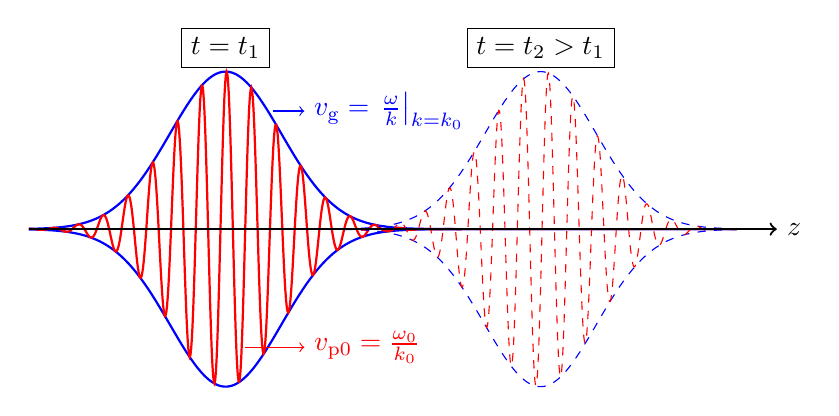
\begin{tikzpicture}[samples=1000, domain=0:9]
	%Plotten
	\draw [color=blue, thick] plot (\x,{exp(-(\x-2.5)^2)*2});
	\draw [color=blue, thick] plot (\x,{-exp(-(\x-2.5)^2)*2});
	\draw [color=red, thick] plot (\x,{cos(deg(\x*20))*exp(-(\x-2.5)^2)*2});

	\draw [style=dashed, color=blue] plot (\x,{exp(-(\x-6.5)^2)*2});
	\draw [style=dashed, color=blue] plot (\x,{-exp(-(\x-6.5)^2)*2});
	\draw [style=dashed, color=red] plot (\x,{cos(deg(\x*20))*exp(-(\x-6.5)^2)*2});

	%\draw[color=red] (0.5,0) sin(0.7,0.5) cos(0.9,0) sin(1.1,-0.66) cos(1.3,0) sin(1.5,1) cos(1.7,0) sin(1.9,-1.37) cos(2.1,0) sin(2.3,1.8) cos(2.5,0) sin(2.7,-2.15) cos(2.9,0) sin(3.1,2.38) cos(3.3,0) sin(3.5,-2.5) cos(3.7,0) sin(3.9,2.38) cos(4.1,0) sin(4.3,-2.15) cos(4.5,0) sin(4.7,1.8) cos(4.9,0) sin(5.1,-1.37) cos(5.3,0) sin(5.5,1) cos(5.7,0) sin(5.9,-0.66) cos(6.1,0) sin(6.3,0.5) cos(6.5,0);
	%\draw (0.5,0.5) cos(2,1.5) sin(3.5,2.5) cos(5,1.5) sin(6.5,0.5);% cos (8,0);
	%\draw (0.5,-0.5) cos(2,-1.5) sin(3.5,-2.5) cos(5,-1.5) sin(6.5,-0.5);% cos (8,0);
	% \begin{axis}
	%        \addplot[samples=500,domain=0:180]{sin(x)*2*sin(20*x)};%x in degrees, 500 samples into the domain
	% \end{axis}

	%Beschriftung
	\draw[->, color=blue] (3.1,1.5)--(3.5,1.5) node[right] {$ v_{\mathrm{g}}=\left.\frac{\dd \omega}{\dd  k}\right|_{ k= k_0}$};
	\draw[->, color=red] (2.75,-1.5)--(3.5,-1.5) node[right] {$ v_{\mathrm{p0}}=\frac{\omega_0}{ k_0}$};
	\node[draw] at (2.5,2.3) {$t=t_1$};
	\node[draw] at (6.5,2.3) {$t=t_2>t_1$};
	% Achse zeichnen
	\draw[->,thick] (0,0) -- (9.5,0) node[right] {$z$};
\end{tikzpicture}